%Preámbulo
\documentclass[11pt, aspectratio = 169]{beamer}
    % Paquetes
    \usepackage{lipsum}
    \usepackage{graphicx}
    \usepackage{float}
    
    %\usetheme{Madrid}
    %\usetheme{CambridgeUS}
    \usetheme{JuanLesPins}
    
    % Título 
    \title{Mi primer beamer}
    \subtitle{Sub título}
    \author{Autor 1 \and Autor 2}
    \institute[UNSCH]{
        {\large Universidad Nacional de San Cristóbal de Huamanga} \\
        {\large Facultad de Ciencias Económicas, Administrativas y Contables}\\
        {\large Escuela Profesional de Economía}
    }
    \date{\today}
    
% Cuerpo
\begin{document}
    % Slide 1.- Llamar el título
    \begin{frame}
        \maketitle
    \end{frame}
    % Slide 2.- Contenido o índice
    \begin{frame}{índice}
        \tableofcontents
    \end{frame}

    % Sección 1
    \section{Introducción}
        % Slide 1.1
        \begin{frame}{Introducción}
            \lipsum[1]
        \end{frame}
    % Sección 2
    \section{Metodología}
        % Slide 2.1
        \begin{frame}
            \frametitle{Metodología}
            \framesubtitle{Modelo econométrico}
            Modelo econométrico de $k$ variables
                \begin{equation}
                    Y_{i} = \beta_{1} + \beta_{2}X_{2i} + \beta_{3}X_{3i} + 
                    \beta_{4}X_{4i} + ... + 
                    \beta_{k}X_{ki}
                \end{equation}
                \begin{equation*}
                    Y_{i} = \beta_{1} + \beta_{2}X_{2i} + \beta_{3}X_{3i} + 
                    \beta_{4}X_{4i} + ... + 
                    \beta_{k}X_{ki}
                \end{equation*}
            Sistema de ecuaciones 
                \begin{align*}
                    a^{2} + b^{2}=&\, c^{2} \\
                    F =&\, ma \\
                    (a + b)^{2} =&\, a^{2} + 2ab + b^{2} 
                \end{align*}
        \end{frame}
        % Slide 2.2
        \begin{frame}
            \frametitle{Metodología}
            \framesubtitle{Figuras}
            \begin{figure}[H]
                \centering
                \caption{Figura 1}
                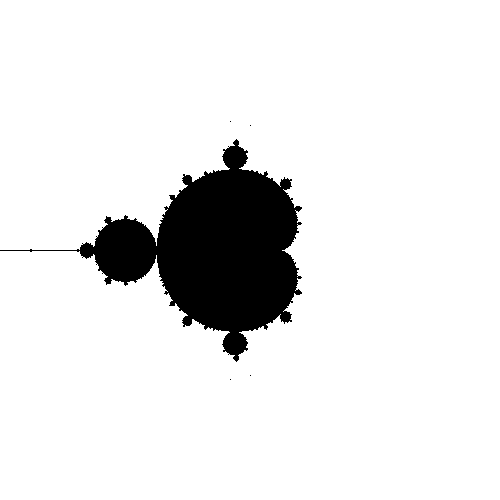
\includegraphics[scale = 0.3]{figura1.png}
            \end{figure}
        \end{frame}
    % Sección 3
    \section{Datos}
        % Slide 3.1
        \begin{frame}{Datos}
            \lipsum[1]
        \end{frame}
    % Sección 4
    \section{Conclusión}
        % Slide 4.1
        \begin{frame}{Conclusión}
            \lipsum[1]. 
        \end{frame}
    % Bibliografía
    \begin{frame}{Bibliografía}
        \bibliography{biblio}
        \bibliographystyle{apalike}
            % Autores
            \nocite{cameron-2010}
    \end{frame}
    % Slide 1.- Llamar el título
    \begin{frame}
        \maketitle
    \end{frame}
    % Appendix
    \begin{frame}{Appendix 1}
        \begin{figure}[H]
            \centering
            \caption{Figura 1}
            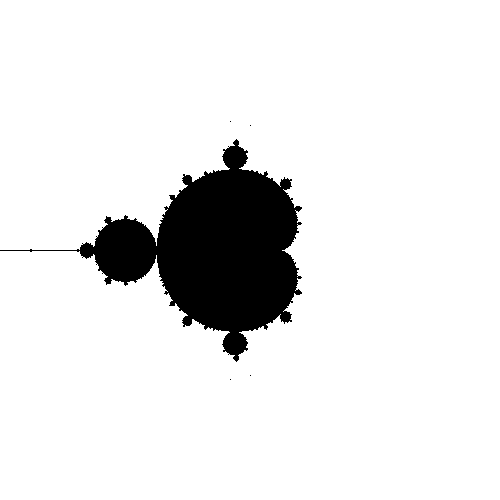
\includegraphics[scale = 0.3]{figura1.png}
        \end{figure}
    \end{frame}
    \begin{frame}{Appendix 2}
        \begin{figure}[H]
            \centering
            \caption{Figura 1}
            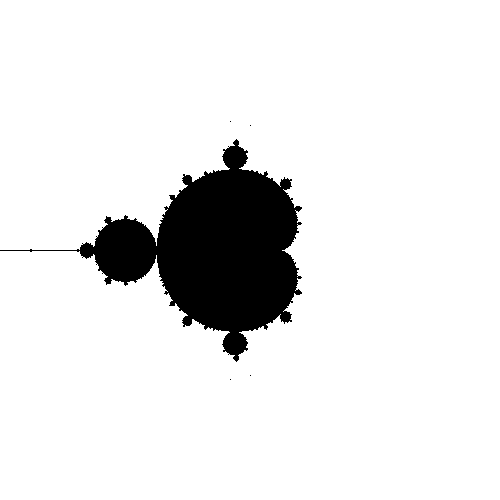
\includegraphics[scale = 0.3]{figura1.png}
        \end{figure}
    \end{frame}
    \begin{frame}{Appendix 3}
        \begin{figure}[H]
            \centering
            \caption{Figura 1}
            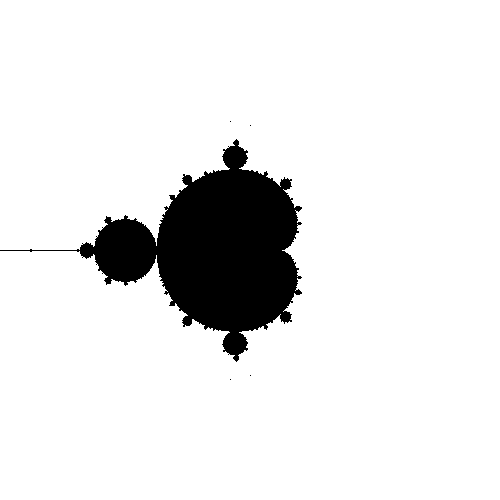
\includegraphics[scale = 0.3]{figura1.png}
        \end{figure}
    \end{frame}
    
\end{document}






